

\section{Reference and Physical Maps}
\label{sec-1}

\label{sec:referenceMaps}

A reference map focuses on the geographic location of features. In
these maps cities are named and major transport routes are
identified. Besides, natural features such as rivers and mountains are
named, and elevation is shown using a simple colour shading.  

A physical map shows the physical landscape features of a
place. Mountains and elevation changes are usually shown with
different colors and shades to show relief, using green to show
lower elevations and browns for high elevations.

This section details how to create a reference map of a northern
region of Spain using data from OpenStreetMap, and a physical map
of Brazil with data from different sources.
\subsection{OpenStreetMap with Hill Shade layers}
\label{sec-1-1}


Although I was born in Madrid, Galicia (north of Spain) is a very
special region for me. More precisely, Cedeira and Valdoviño
regions offer a wonderful combination of wild sea, secluded
beaches and forests. I will show you a map of these marvelous
places.

The first step is to acquire information from the OpenStreetMap
project. There are several packages to extract data from this
service but, while most of them only provide already rendered
raster images, the \texttt{osmar} package\footnote{Its webpage \href{http://osmar.r-forge.r-project.org/}{http://osmar.r-forge.r-project.org/} proposes
  two interesting demos.
 } enables the use of the raw data
with classes from the packages \texttt{sp} and \texttt{igraph}.

The \texttt{get\_osm} function retrieves a region defined by \texttt{corner\_bbox}
using the OSM API.

\index{Data!OpenStreetMap}
\index{Packages!osmar@\texttt{osmar}}
\index{osmsource_api@\texttt{osmsource\_api}}
\index{get_osm@\texttt{get\_osm}}

\lstset{language=R}
\begin{lstlisting}
library('osmar')

api <- osmsource_api()
ymax <- 43.7031
ymin <- 43.6181
xmax <- -8.0224
xmin <- -8.0808
box <- corner_bbox(xmin, ymin, xmax, ymax)
cedeira <- get_osm(box, source=api, full=TRUE)
summary(cedeira)
\end{lstlisting}


\begin{verbatim}
osmar object
5927 nodes, 148 ways, 7 relations 

osmar$nodes object
5927 nodes, 2702 tags 

..$attrs data.frame: 
    id, lat, lon, user, uid, visible, version, changeset, timestamp 
..$tags data.frame: 
    id, k, v 
 
Bounding box:
         lat       lon
min 43.53471 -8.149651
max 43.75000 -7.883569

Key-Value contingency table:
         Key                   Value Freq
1     source                     PGS  661
2 created_by almien_coastlines mo...  548
3 created_by                    JOSM  441


osmar$ways object
148 ways, 238 tags, 6108 refs 

..$attrs data.frame: 
    id, user, uid, visible, version, changeset, timestamp 
..$tags data.frame: 
    id, k, v 
..$refs data.frame: 
    id, ref 
 
Key-Value contingency table:
      Key        Value Freq
1 highway  residential   71
2 highway unclassified   27
3  source          PGS   17


osmar$relations object
7 relations, 106 tags, 5 node_refs, 1824 way_refs 

..$attrs data.frame: 
    id, user, uid, visible, version, changeset, timestamp 
..$tags data.frame: 
    id, k, v 
..$refs data.frame: 
    id, type, ref, role 
 
Key-Value contingency table:
       Key                   Value Freq
1 boundary          administrative    6
2     type                boundary    6
3   source BDLL25, EGRN, Instit...    5
\end{verbatim}

The \texttt{cedeira} object includes three main components: nodes, ways
and relations. 
  

\lstset{language=R}
\begin{lstlisting}
summary(cedeira$nodes)
\end{lstlisting}


\begin{verbatim}
osmar$nodes object
5927 nodes, 2702 tags 

..$attrs data.frame: 
    id, lat, lon, user, uid, visible, version, changeset, timestamp 
..$tags data.frame: 
    id, k, v 
 
Bounding box:
         lat       lon
min 43.53471 -8.149651
max 43.75000 -7.883569

Key-Value contingency table:
                Key                   Value Freq
1            source                     PGS  661
2        created_by almien_coastlines mo...  548
3        created_by                    JOSM  441
4            source Instituto Geográfico...   44
5  is_in:state_code                      15   42
6       source:date                  201011   42
7         ngbe:huso                      29   42
8       ngbe:codigo                   80214   42
9       source:file http://centrodedesca...   42
10             note If you change this n...   42
\end{verbatim}

These components can be accessed with the functions \texttt{find}, \texttt{subset}, \texttt{way},
\texttt{node}, \texttt{relation} and \texttt{tags}. Thus, the different kinds of roads
can be obtained using \texttt{way} and \texttt{tags} with the appropiate
tag. 

\index{find@\texttt{find}}
\index{subset@\texttt{subset}}
\index{way@\texttt{way}}

\lstset{language=R}
\begin{lstlisting}
idxHighways <- find(cedeira, way(tags(k=='highway')))
highways <- subset(cedeira, way_ids=idxHighways)
idxStreets <- find(highways, way(tags(v=='residential')))
idxPrimary <- find(highways, way(tags(v=='primary')))
idxSecondary <- find(highways, way(tags(v=='secondary')))
idxTertiary <- find(highways, way(tags(v=='tertiary')))
idxOther <- find(highways,
                 way(tags(v=='unclassified' |
                          v=='footway' |
                          v=='steps')))
\end{lstlisting}

The result of \texttt{find} is the index of each element. The
correspondent spatial object is extracted with \texttt{find\_down} and
\texttt{subset}, and can be converted to a class defined by the \texttt{sp}
package with \texttt{as\_sp}. The next \texttt{spFromOSM} function encodes the
procedure, and extracts the \texttt{SpatialLines} which represent each
type of road.

\index{as_sp@\texttt{as\_sp}}
\index{find_down@\texttt{find\_down}}

\lstset{language=R}
\begin{lstlisting}
spFromOSM <- function(source, index, type='lines'){
  idx <- find_down(source, index)
  obj <- subset(source, ids=idx)
  objSP <- as_sp(obj, type)
  }

streets <- spFromOSM(cedeira, way(idxStreets))
primary <- spFromOSM(cedeira, way(idxPrimary))
secondary <- spFromOSM(cedeira, way(idxSecondary))
tertiary <- spFromOSM(cedeira, way(idxTertiary))
other <- spFromOSM(cedeira, way(idxOther))
\end{lstlisting}
  
A similar procedure can be applied to construct a \texttt{SpatialPoints}
object with the collection of places with name:

\index{match\texttt{match}}

\lstset{language=R}
\begin{lstlisting}
idxPlaces <- find(cedeira, node(tags(k=='name')))
places <- spFromOSM(cedeira, node(idxPlaces), 'points')

nms <- subset(cedeira$nodes$tags, subset=(k=='name'), select=c('id', 'v'))
ord <- match(idxPlaces, nms$id)
nms <- nms[ord,]
places$name <- nms$v[ord]

## Cedeira town will be printed differently
idxCedeira <- which(nms$v=='Cedeira') ##Main town
cedeiraCoords <- coordinates(places[idxCedeira,])
places <- places[-idxCedeira,]
\end{lstlisting}

\index{Hill shading}

The second step is to produce layers to display the topography. A
suitable method is the shaded relief or hill shading. This
technique simulate the cast shadow thrown from a light source upon
a raised relief map. The hill shade layer can be computed from the
slope and aspect layers derived from a Digital Elevation
Model. This layer will underlay the DEM raster, which will be printed
using semitransparency.  

The DEM for this region is available at
the Geonetwork-SECAD service from the Universidad de Extremadura
and can be read with \texttt{raster}:

\index{Packages!raster@\texttt{raster}}
\index{Packages!rasterVis@\texttt{rasterVis}}
\index{Data!Geonetwork}

\lstset{language=R}
\begin{lstlisting}
library(raster)
## Galicia DEM
## http://ide.unex.es/geonetwork/srv/es/main.search?any=MDE_Galicia
## http://ide.unex.es:8180/geonetwork/srv/es/resources.get?id=21&fname=dem_gal.7z&access=private

old <- tempdir()
download.file('http://ide.unex.es:8180/geonetwork/srv/es/resources.get?id=21&fname=dem_gal.7z&access=private', 'dem_gal.7z')
unzip('dem_gal.7z')
demGalicia <- raster('dem_gal.asc')
setwd(old)
\end{lstlisting}



The \texttt{slope} and \texttt{aspect} layers are computed with the \texttt{terrain}
function, and the hill shade layer is derived with these layers
for a fixed sun position. Previously, the useful region of the DEM
raster is extracted with the \texttt{crop} function:

\index{terrain@\texttt{terrain}}
\index{crop@\texttt{crop}}
\index{hillShade@\texttt{hillShade}}
\index{Hill shading}

\lstset{language=R}
\begin{lstlisting}
cedeiraSP <- as_sp(cedeira, 'points')
projCedeira <- projection(cedeiraSP)
##extCedeira <- bbox(cedeiraSP) 
## or summary(cedeira$nodes)$bbox
extCedeira <- extent(-8.15, -7.95, 43.6, 43.75)
demCedeira <- crop(demGalicia, extCedeira)
projection(demCedeira) <- projCedeira
demCedeira[demCedeira <= 0] <- NA

slope <- terrain(demCedeira, 'slope')
aspect <- terrain(demCedeira, 'aspect')
hsCedeira <- hillShade(slope=slope, aspect=aspect,
                       angle=20, direction=30)
\end{lstlisting}

And finally, the third step is to display the different layers of
information in correct order (figure \ref{fig:cedeiraOsmar}):

\begin{itemize}
\item The hill shade layer is created with the \texttt{levelplot} method for
  \texttt{Raster} objects defined in the \texttt{rasterVis} package. The
  \texttt{GrTheme} is modified to display the sea region with blue color.
\item The DEM raster is printed with terrain colors and
  semitransparency over the hill shade layer.
\item The roads are displayed with an auxiliary function (\texttt{sp.road})
  which produces a colored line over a thicker black line.
\item The places are represented with \texttt{sp.points} and labelled with
  the \texttt{sp.pointLabel} method, a modification of the \texttt{pointLabel}
  function for \texttt{base} graphics, both defined in the \texttt{maptools}
  package. These functions use optimization routines to find good
  locations for point labels without overlaps.
\end{itemize}

\index{Packages!maptools@\texttt{maptools}}  
\index{Packages!sp@\texttt{sp}}  
\index{Packages!latticeExtra@\texttt{latticeExtra}}  
\index{Packages!colorspace@\texttt{colorspace}}  
\index{sp.lines@\texttt{sp.lines}}
\index{sp.lines@\texttt{sp.points}}
\index{sp.lines@\texttt{sp.pointLabel}}

\lstset{language=R}
\begin{lstlisting}
library(maptools)
library(latticeExtra)
library(colorspace)
library(rasterVis)

##Auxiliary function to display the roads. A thicker black line in
##the background and a thinner one with an appropiate color.
sp.road <- function(line, lwd=5, blwd=7,
                    col='indianred1', bcol='black'){
  sp.lines(line, lwd=blwd, col=bcol)
  sp.lines(line, lwd=lwd, col=col)
}

## The background color of the panel is set to blue to represent the sea
hsTheme <- modifyList(GrTheme(), list(panel.background=list(col='skyblue3')))
## DEM with terrain colors and semitransparency
terrainTheme <- modifyList(rasterTheme(region=terrain_hcl(n=15)),
                                list(regions=list(alpha=0.6)))
## Hill shade and DEM overlaid
levelplot(hsCedeira, maxpixels=ncell(hsCedeira),
          par.settings=hsTheme, margin=FALSE, colorkey=FALSE) +
  levelplot(demCedeira, maxpixels=ncell(demCedeira),
            par.settings=terrainTheme) +
  ## Roads and places
  layer({
    ## Street and roads
    sp.road(streets, lwd=1, blwd=2, col='white')
    sp.road(other, lwd=2, blwd=3, col='white')
    sp.road(tertiary, lwd=3, blwd=4, col='palegreen')
    sp.road(secondary, lwd=4, blwd=6, col='midnightblue')
    sp.road(primary, col='indianred1')
    ## Places except Cedeira town
    sp.points(places, pch=19, col='black', cex=0.4, alpha=0.8)
    sp.pointLabel(places, labels=places$name,
                      fontfamily = 'Palatino', 
                      cex=0.6, col='black')
    ## Cedeira town
    panel.points(cedeiraCoords, pch=18, col='black', cex=1)
    panel.text(cedeiraCoords, labels='Cedeira', pos=2, offset=1)
    })
\end{lstlisting}

\begin{figure}[htb]
\centering
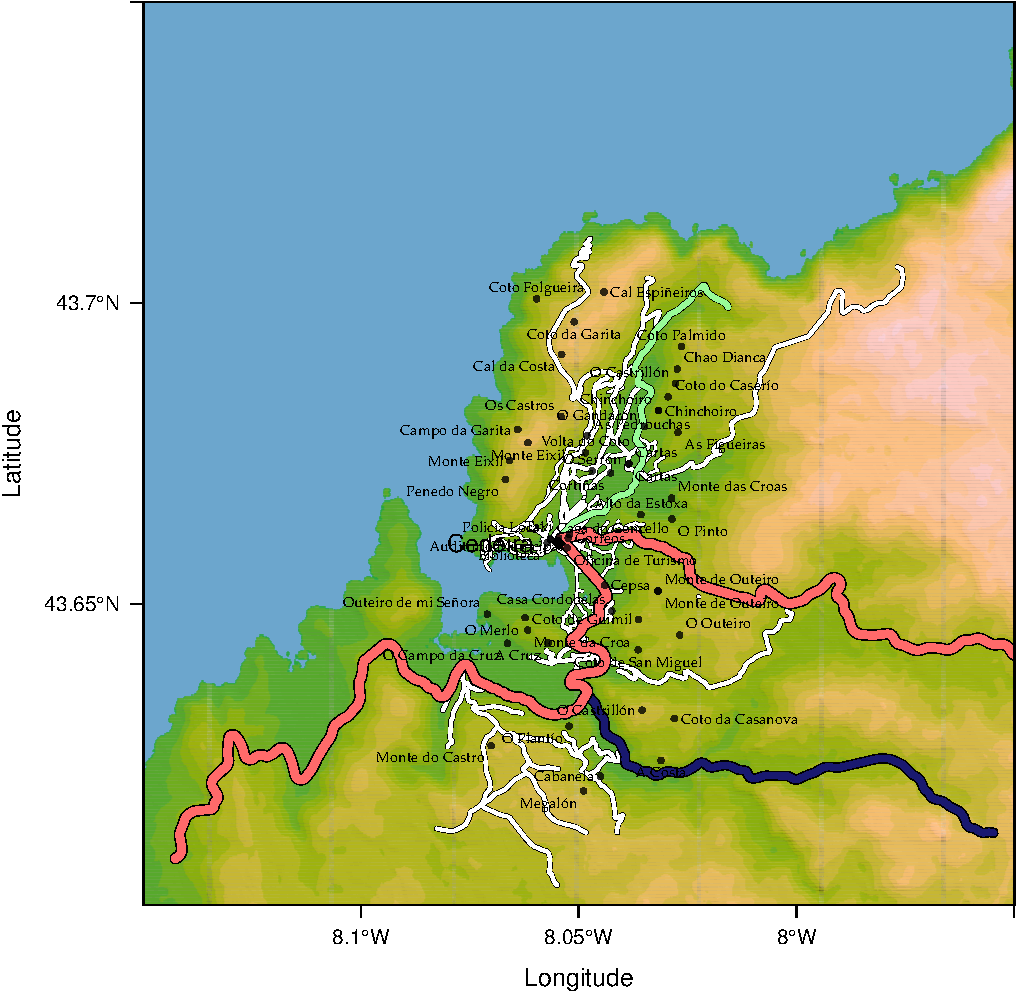
\includegraphics[width=.9\linewidth]{figs/cedeiraOsmar.pdf}
\caption{\label{fig:cedeiraOsmar}Main roads near Cedeira, Galicia. Local topography is displayed with the hill shading technique. Some places are highlighted.}
\end{figure}
\subsection{Brazil}
\label{sec-1-2}


Brazil\footnote{http://en.wikipedia.org/wiki/Brazil
 }, the world's fifth largest country, is one of the 17
megadiverse countries\footnote{http://en.wikipedia.org/wiki/Megadiverse\_{}countries
 }, home to diverse wildlife, natural
environments, and extensive natural resources in a variety of
protected habitats. Throughout this section we will create a physical
map of this exceptional country using data from the
DIVA-GIS\footnote{http://www.diva-gis.org/Data
 }, GADM\footnote{http://gadm.org/
 } and Natural Earth Data\footnote{http://www.naturalearthdata.com/
 } projects.

\index{Packages!raster@\texttt{raster}}  
\index{Packages!rasterVis@\texttt{rasterVis}}  
\index{Packages!sp@\texttt{sp}}  
\index{Packages!maptools@\texttt{maptools}}  
\index{Packages!colorspace@\texttt{colorspace}}  

\lstset{language=R}
\begin{lstlisting}
library(raster)
library(rasterVis)
library(maptools)
library(latticeExtra)
library(colorspace)
\end{lstlisting}

\index{CRS@\texttt{CRS}}
\index{download.file@\texttt{download.file}}
\index{readShapePoly@\texttt{readShapePoly}}
\index{readShapeLines@\texttt{readShapeLines}}
\index{Encoding@\texttt{Encoding}}
\index{raster@\texttt{raster}}
\index{Data!GADM}
\index{Data!DIVA-GIS}
\index{Data!Natura Earth Data}

\lstset{language=R}
\begin{lstlisting}
old <- setwd(tempdir())

## Longitude-Latitude projection
proj <- CRS(' +proj=longlat +ellps=WGS84')

## Administrative boundaries (GADM)
download.file('http://www.gadm.org/data/shp/BRA_adm.zip', 'BRA_adm.zip')
unzip('BRA_adm.zip')
brazilAdm <- readShapePoly('BRA_adm1.shp', proj4string=proj)
Encoding(levels(brazilAdm$NAME_1)) <- 'latin1'

## Altitude raster (DIVA-GIS)
download.file('http://www.diva-gis.org/data/alt/BRA_alt.zip', 'BRA_alt.zip')
unzip('BRA_alt.zip')
brazilAlt <- raster('BRA_alt')

## World Water lines (Natural Earth)
download.file('http://www.naturalearthdata.com/http//www.naturalearthdata.com/download/10m/physical/ne_10m_rivers_lake_centerlines.zip', 'neRivers.zip')
unzip('neRivers.zip')
worldlRiv <- readShapeLines('ne_10m_rivers_lake_centerlines', proj4string = proj)

## Sea depth (Natural Earth)
download.file('http://www.naturalearthdata.com/http//www.naturalearthdata.com/download/10m/raster/OB_LR.zip', 'neSea.zip')
unzip('neSea.zip')
worldSea <- raster('OB_LR.tif')
brazilSea <- crop(worldSea, brazilAlt)

setwd(old)
\end{lstlisting}

The rivers and lakes database from Natural Earth Data comprises
all the world extent. With a helper function, the extent of each
line is calculated and compared with the \texttt{brazilAlt} raster
extent. Those lines contained in this extent are included in a new
\texttt{brazilRiv} object. 
\index{intersect@\texttt{intersect}}
\index{extent@\texttt{extent}}
\index{lapply@\texttt{lapply}}

\lstset{language=R}
\begin{lstlisting}
## only those features labelled as "River" are needed
worlRiv<- worlRiv[worlRiv$featurecla=='River',]

## Helper function that calculates the extent of a line to crop it
## with an extent object using intersect
extentLine <- function(line){
  bb <- bbox(line)
  e <- extent(c(bb[1,1], bb[1,2], bb[2,1], bb[2,2]))
  e
}

extBrazil <- extent(brazilAlt)
## For each line test if it is inside Brazil
intersectBrazil <- lapply(worlRiv@lines, function(line){
  extLine <- extentLine(line)
  int <- intersect(extentLine(line), extBrazil)
})

inBrazil <- which(sapply(intersectBrazil, function(x)!is.null(x)))
## Extract rivers from the world database
brazilRiv <- worlRiv[inBrazil,]
## and specially the famous Amazonas River
amazonas <- brazilRiv[brazilRiv$name=='Amazonas',]
\end{lstlisting}



Each region of Brazil will be labelled with the name of its
correspondent polygon. The locations of the labels are defined by the
centroid of each polygon, easily computed with the \texttt{coordinates}
method. Besides, a larger label with the name of the country will be
placed in the average centroid.

\index{coordinates@\texttt{coordinates}}
\index{apply@\texttt{apply}}

\lstset{language=R}
\begin{lstlisting}
## Locations of labels of each polygon
centroids <- coordinates(brazilAdm)
## Location of the "Brazil" label (average of the set of polygons centroids)
xyBrazil <- apply(centroids, 2, mean)
\end{lstlisting}

Some region names are too long to be displayed in one line. Thus, a
previous step is to split the string if it comprises more than 2
words.
\index{sapply@\texttt{sapply}}
\index{strsplit@\texttt{strsplit}}

\lstset{language=R}
\begin{lstlisting}
admNames <- strsplit(as.character(brazilAdm$NAME_1), ' ')

admNames <- sapply(admNames,
                 FUN=function(s){
                   sep=if (length(s)>2) '\n' else  ' '
                   paste(s, collapse=sep)
                   })
\end{lstlisting}


  
  
  
  


Therefore, the physical map (figure \ref{fig:brazil} is composed
of four layers: 

\begin{itemize}
\item The sea depth raster displayed with the \texttt{levelplot} method of
  the \texttt{rasterVis} package. For this layer the \texttt{Blues} palette
  produced with \texttt{brewer.pal} is chosen.
\end{itemize}

\index{rasterTheme@\texttt{rasterTheme}}
\index{brewer.pal@\texttt{brewer.pal}}

\lstset{language=R}
\begin{lstlisting}
blueTheme <- rasterTheme(region=brewer.pal(n=9, 'Blues'))
\end{lstlisting}

\begin{itemize}
\item The altitude raster layer with a terrain colors palette, as the
  one produced by the \texttt{terrain\_hcl} function from the \texttt{colorspace}
  package.
\end{itemize}

\index{rasterTheme@\texttt{rasterTheme}}
\index{terrain_hcl@\texttt{terrain\_hcl}}

\lstset{language=R}
\begin{lstlisting}
terrainTheme <- rasterTheme(region=terrain_hcl(15))
\end{lstlisting}

\begin{itemize}
\item The rivers represented by a \texttt{SpatialLines} object. The Amazonas
  river is labelled with \texttt{sp.lineLabel} and printed with a thicker
  line.
\item The administrative boundaries represented by an \texttt{SpatialPolygons}
  object with their labels printed with the \texttt{panel.text} function.
\end{itemize}


\index{levelplot@\texttt{levelplot}}
\index{sp.lines@\texttt{sp.lines}}
\index{sp.lineLabel@\texttt{sp.lineLabel}}
\index{sp.polygons@\texttt{sp.polygons}}
\index{panel.text@\texttt{panel.text}}
\index{layer@\texttt{layer}}
\index{brewer.pal@\texttt{brewer.pal}}

\lstset{language=R}
\begin{lstlisting}
labs <- label(amazonas, 'Amazonas')

seaPlot <- levelplot(brazilSea, par.settings=blueTheme,
                     maxpixels=1e6, panel=panel.levelplot.raster,
                     margin=FALSE, colorkey=FALSE)

altPlot <- levelplot(brazilAlt, par.settings=terrainTheme,
                     maxpixels=1e6, panel=panel.levelplot.raster,
                     margin=FALSE, colorkey=FALSE)

seaPlot + altPlot + layer({
  sp.lines(brazilRiv, col='darkblue', lwd=0.3)

  sp.lineLabel(amazonas, labs, 
               lwd=1.3, col='darkblue', col.line='darkblue',
               cex=0.5, fontfamily='Palatino')


  sp.polygons(brazilAdm, col='black', lwd=0.5)
  panel.text(coordinates(brazilAdm), labels=admNames,
             cex=0.5, fontfamily='Courier', lineheight=.8)

  panel.text(xyBrazil[1], xyBrazil[2], labels='B R A Z I L',
             cex=1.5, fontfamily = 'Palatino', fontface=2)
  })
\end{lstlisting}

\begin{figure}[htb]
\centering
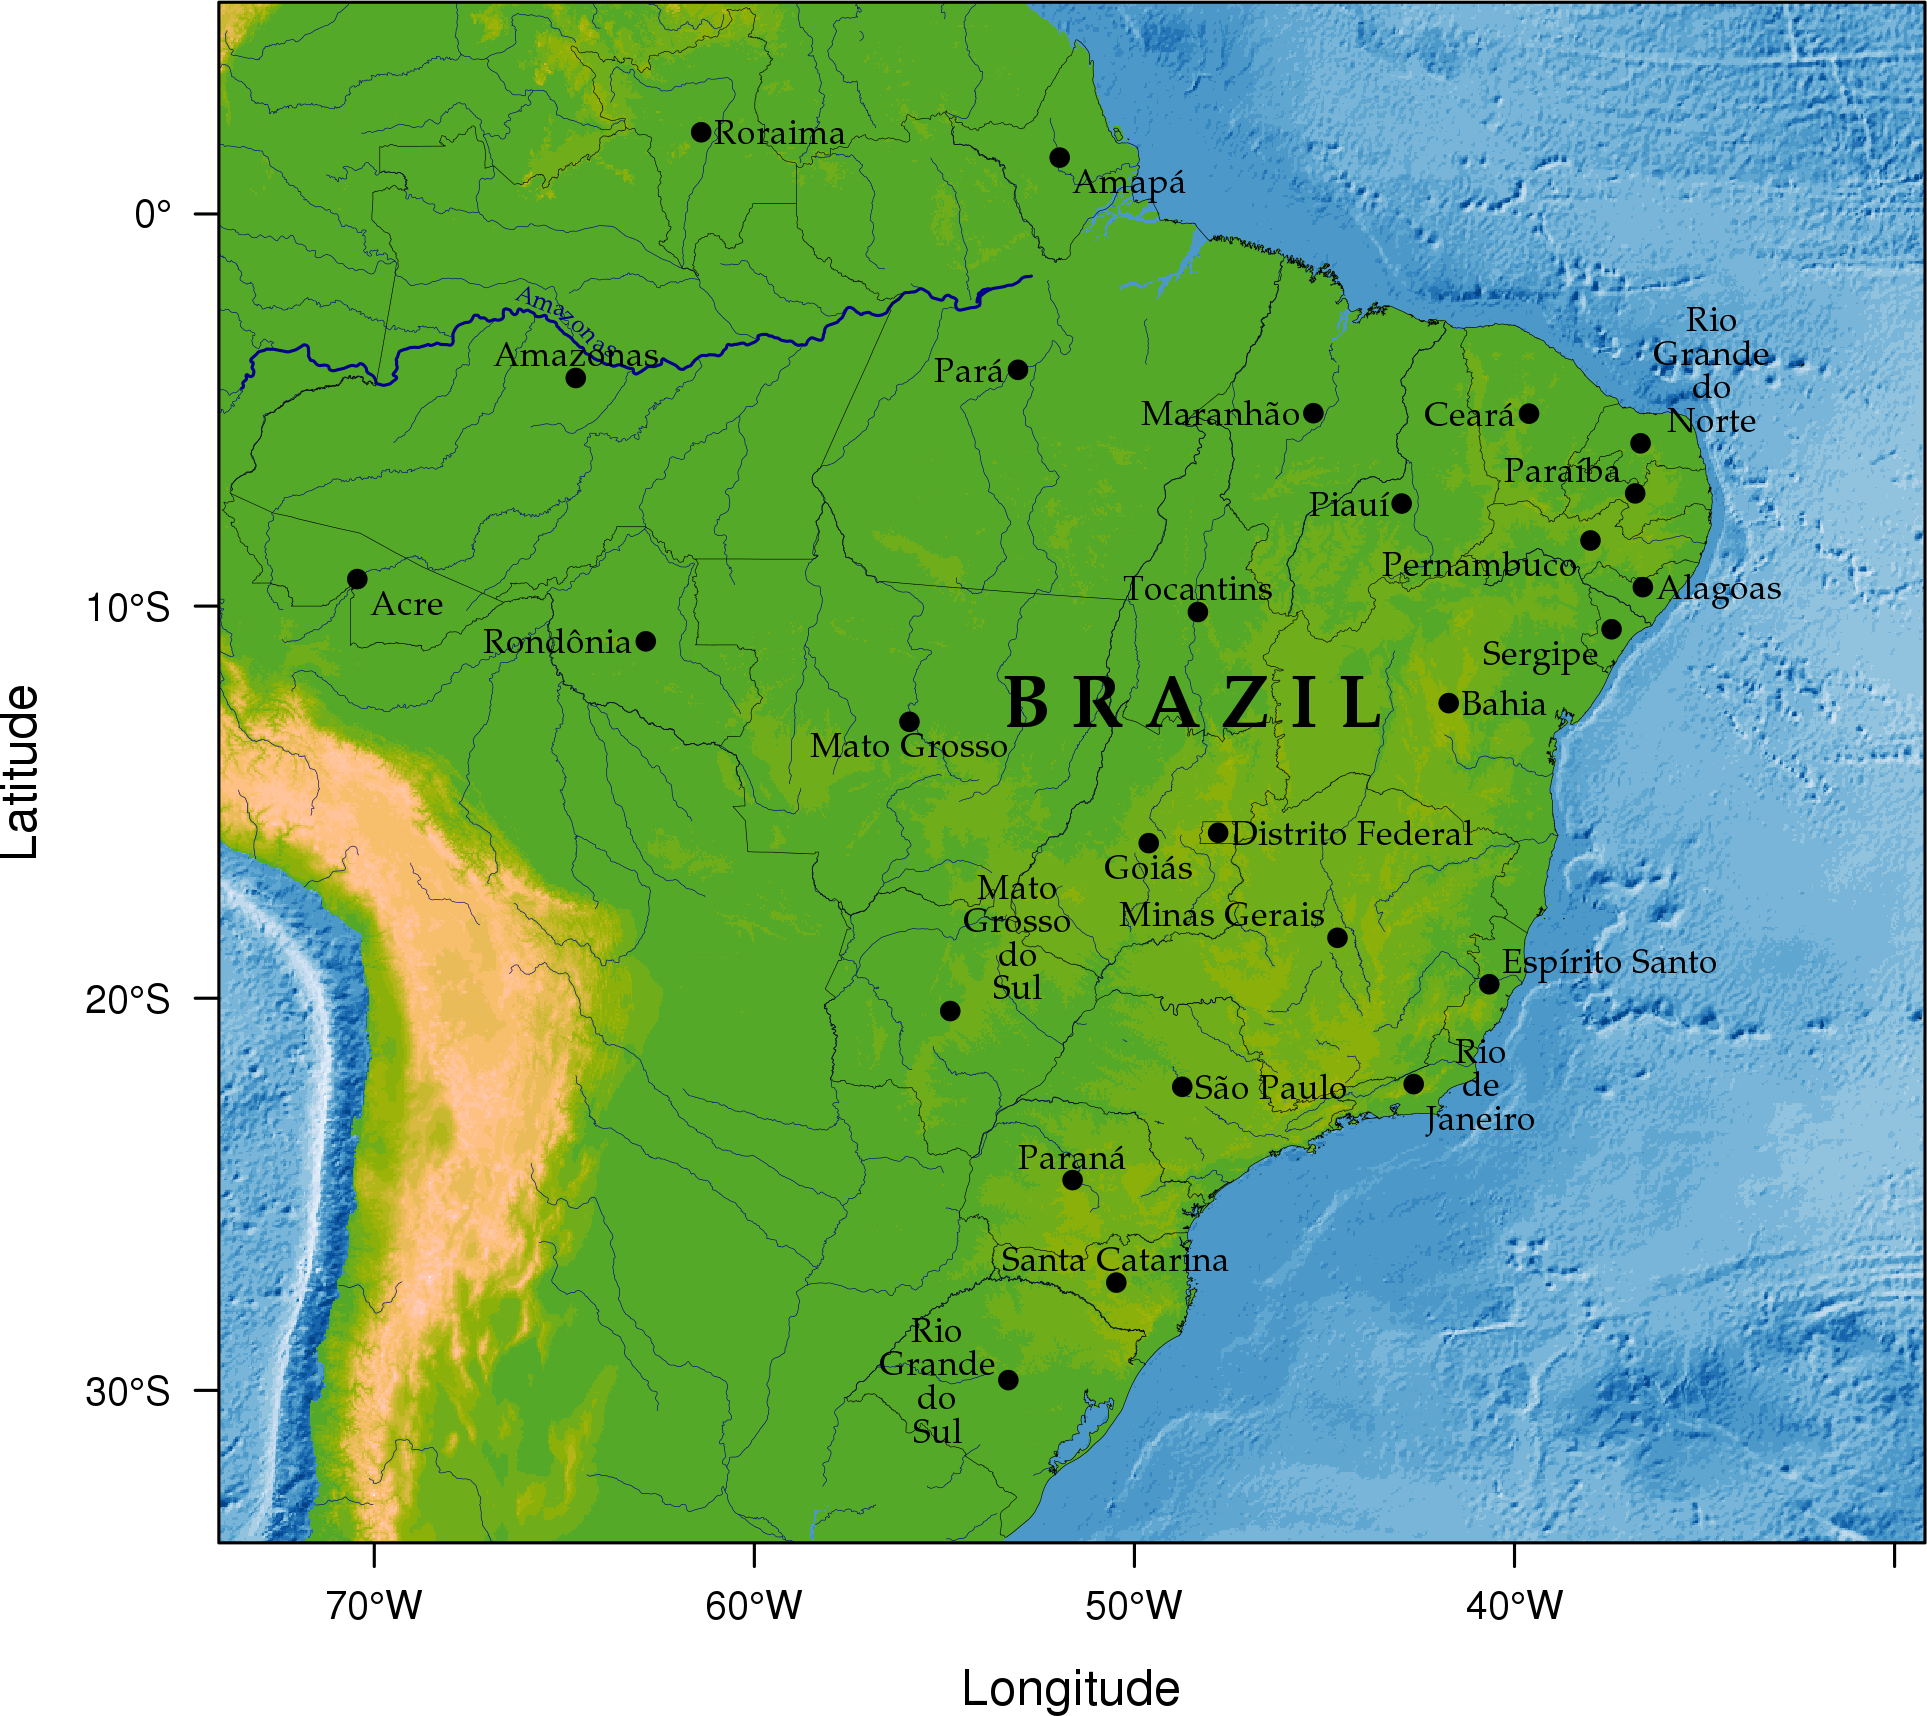
\includegraphics[width=.9\linewidth]{figs/brazil.pdf}
\caption{\label{fig:brazil}Physical map of Brazil. Main administrative regions and the Amazonas river are labelled.}
\end{figure}
